\documentclass[class=beamer, crop=false]{standalone}
%packages
\usepackage[subpreambles=true]{standalone}
\usepackage{import}
\usepackage[utf8]{inputenc}
\usepackage[T1]{fontenc}
\usepackage[naustrian]{babel}
\usepackage{color}
\usepackage{graphicx}
\usepackage{minted}
\usepackage{url}
\usepackage{framed}
%title
\title{JDBC – Java Database Connectivity \\ Einführung}
\author{Lukas Wais}
\institute{Codersbay}
\date{\today}
%\pgfpagesuselayout{}[a4paper]
%Information to be included in the title page:

%theme
\usetheme{Berlin}
%\setbeamercolor*{palette primary}{bg=black, fg = white}
%\setbeamercolor*{palette secondary}{bg=black, fg = white}
%\setbeamercolor*{palette tertiary}{bg=gray, fg = white}
%\setbeamercolor*{palette quaternary}{bg=black, fg = white}

\begin{document}
\frame{\titlepage}

\begin{frame}
	\frametitle{Inhaltsverzeichnis}
	\tableofcontents
\end{frame}

\section{Was ist JDBC?}
\subsection{Einführung}

\begin{frame}
	\frametitle{Overview}
	\framesubtitle{Datenbank APIs ohne JDBC}
	\begin{center}
	\begin{figure}
  		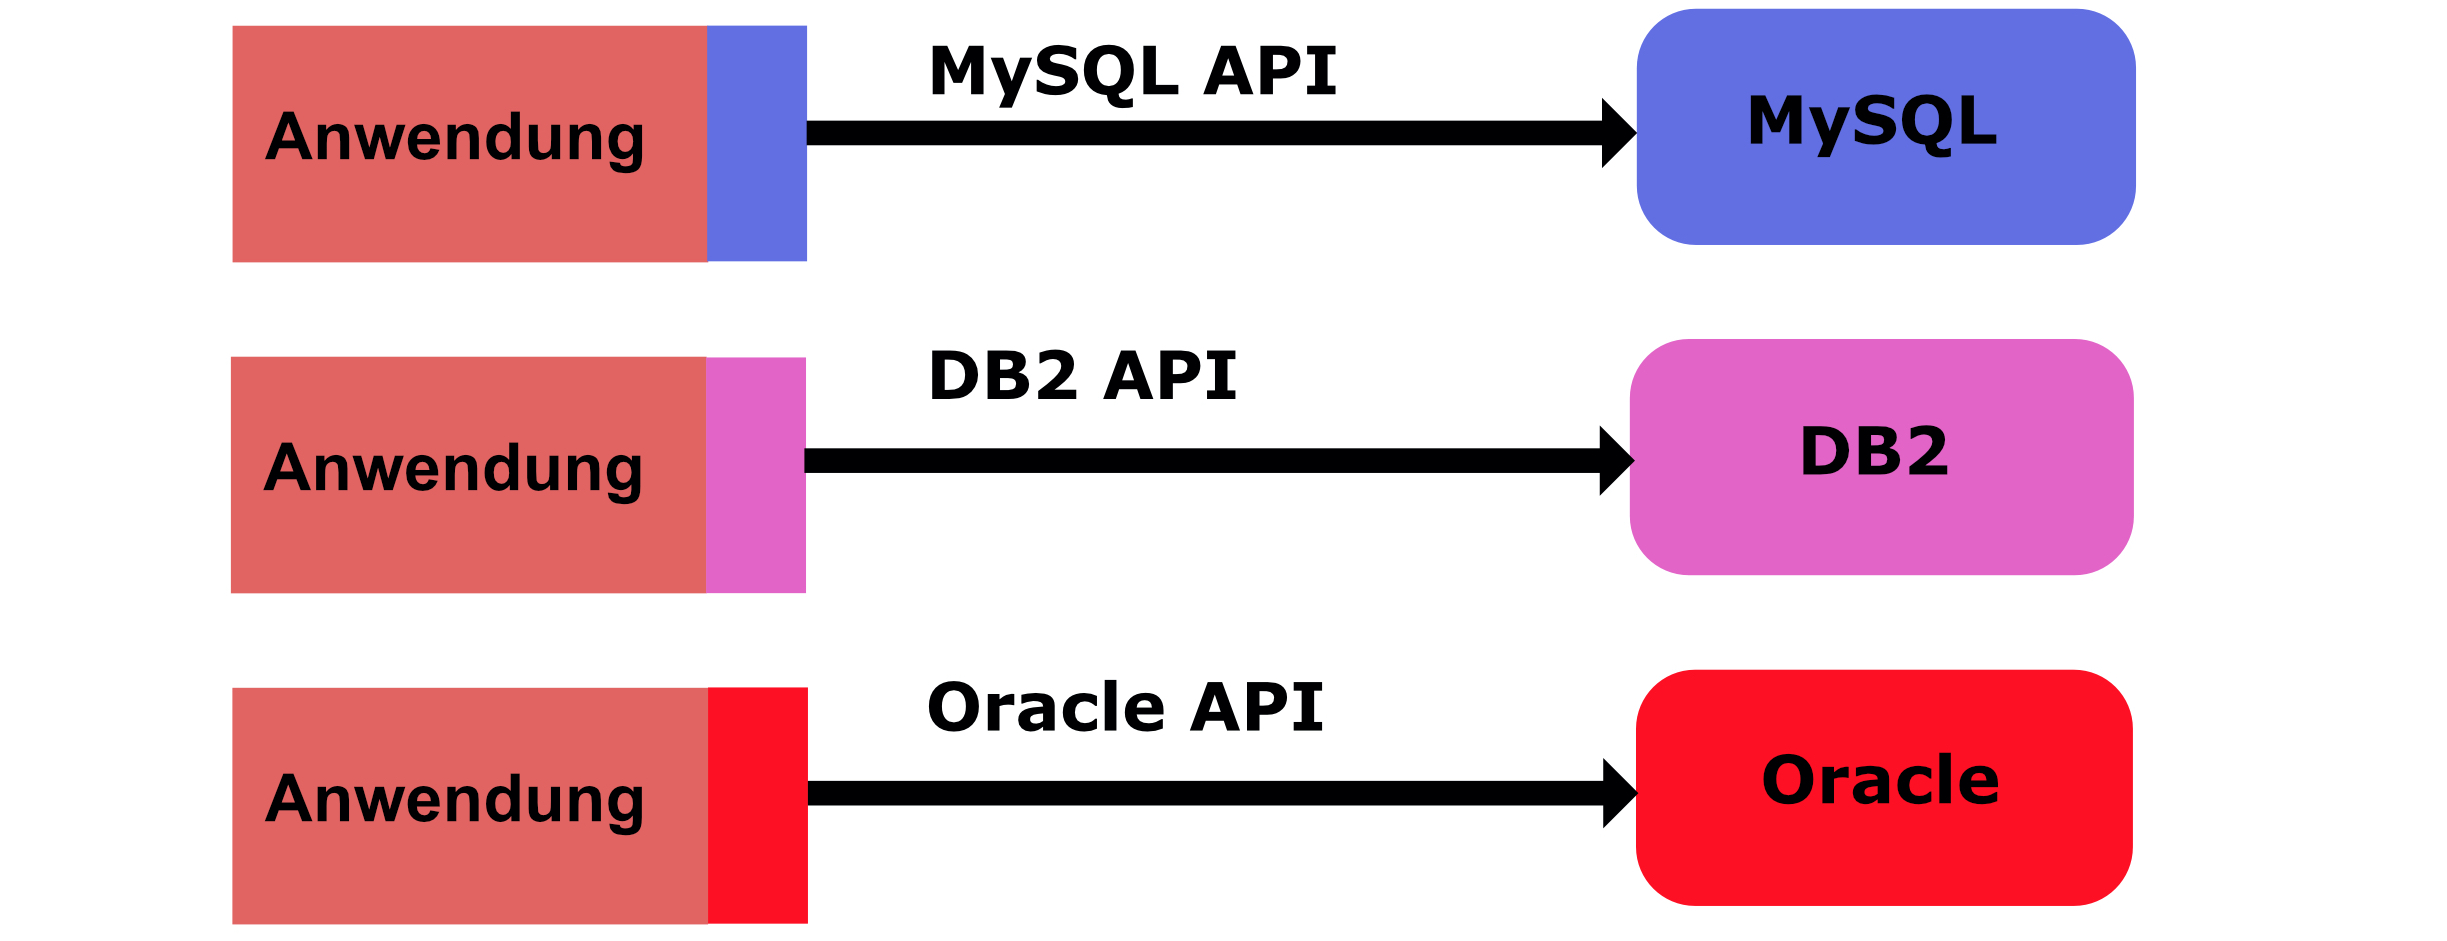
\includegraphics[width=\linewidth]{./img/apis.jpg}
  		\caption{Datenbank APIs ohne JDBC}
  		\label{Datenbank APIs ohne JDBC}
	\end{figure}
	\end{center}
	API $\ldots$ Application Programming Interface
\end{frame}

\begin{frame}
	\frametitle{Overview}
	\framesubtitle{Datenbank APIs ohne JDBC}
	\begin{center}
	\begin{figure}
  		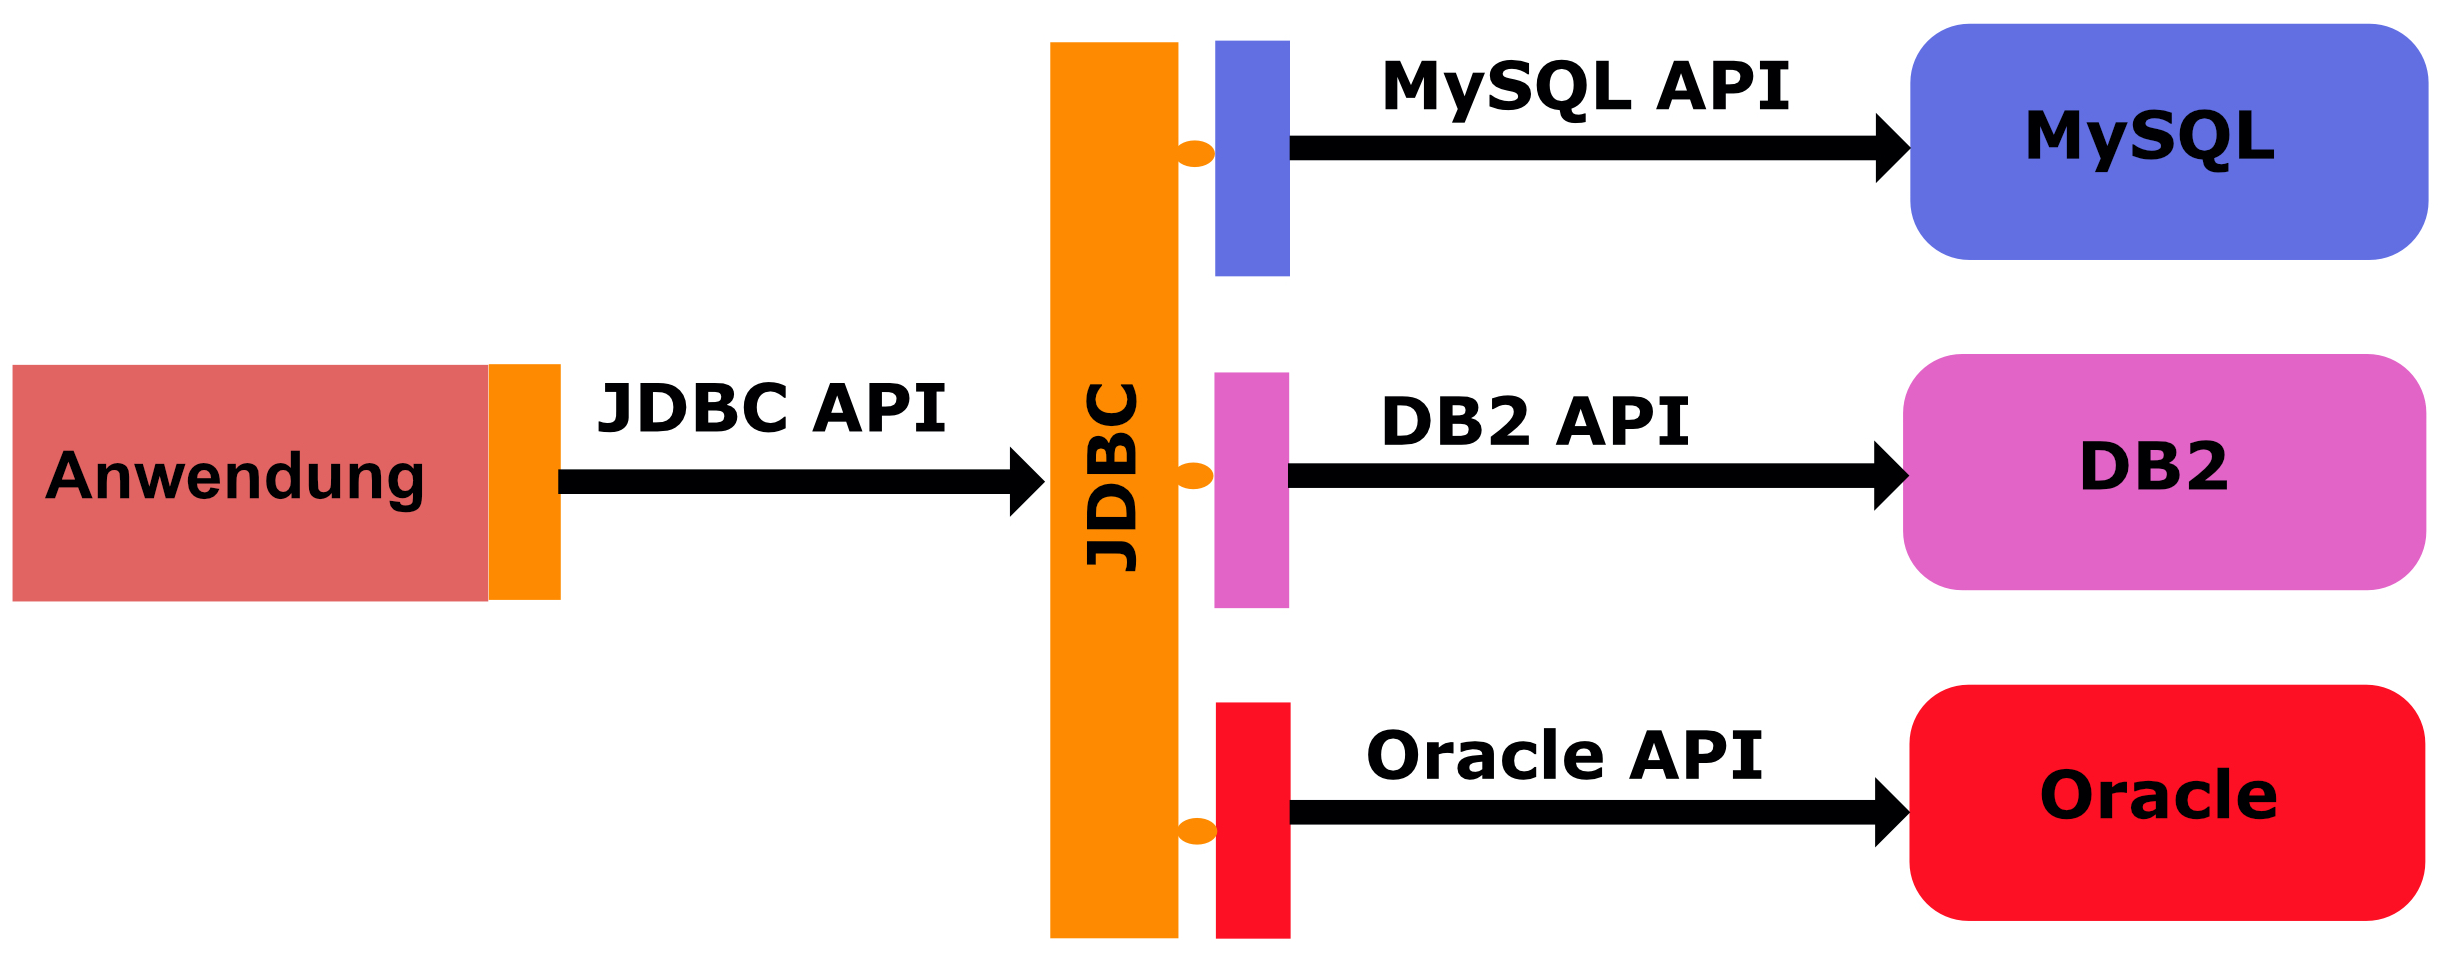
\includegraphics[width=\linewidth]{./img/apisJDBC.jpg}
  		\caption{Datenbank APIs mit JDBC}
  		\label{Datenbank APIs mit JDBC}
	\end{figure}
	\end{center}
\end{frame}

\begin{frame}
	\frametitle{Datenbankzugriffsschnittstelle für Java}
	\begin{itemize}
		\item abstrakt und datenbankneutral
		\item vergleichbar mit ODBC
		\item \textcolor{red}{Low-Level-API: direkte Nutzung von SQL}
		\item Java-Package java.sql
		\item entwickelt von Sun Microsystems
	\end{itemize}
\end{frame}

\begin{frame}
	\frametitle{Klassen}
	\begin{itemize}
		\item \textbf{DriverManager:} Einstiegspunkt, Laden von Treibern
		\item \textbf{Connection:} Datenbankverbindung
		\item \textbf{Statement:} Ausführung von Anweisungen über eine Verbindung
		\item \textbf{ResultSet:} verwaltet Ergebnisse einer Anfrage, Zugriff auf einzelne Spalten
	\end{itemize}
\end{frame}

\section{Verbindung}
\subsection{Ablauf}
\begin{frame}
	\frametitle{Ablauf der Datenbankverbindung}
	\framesubtitle{Diagramm}
	\begin{center}
	\begin{figure}
  		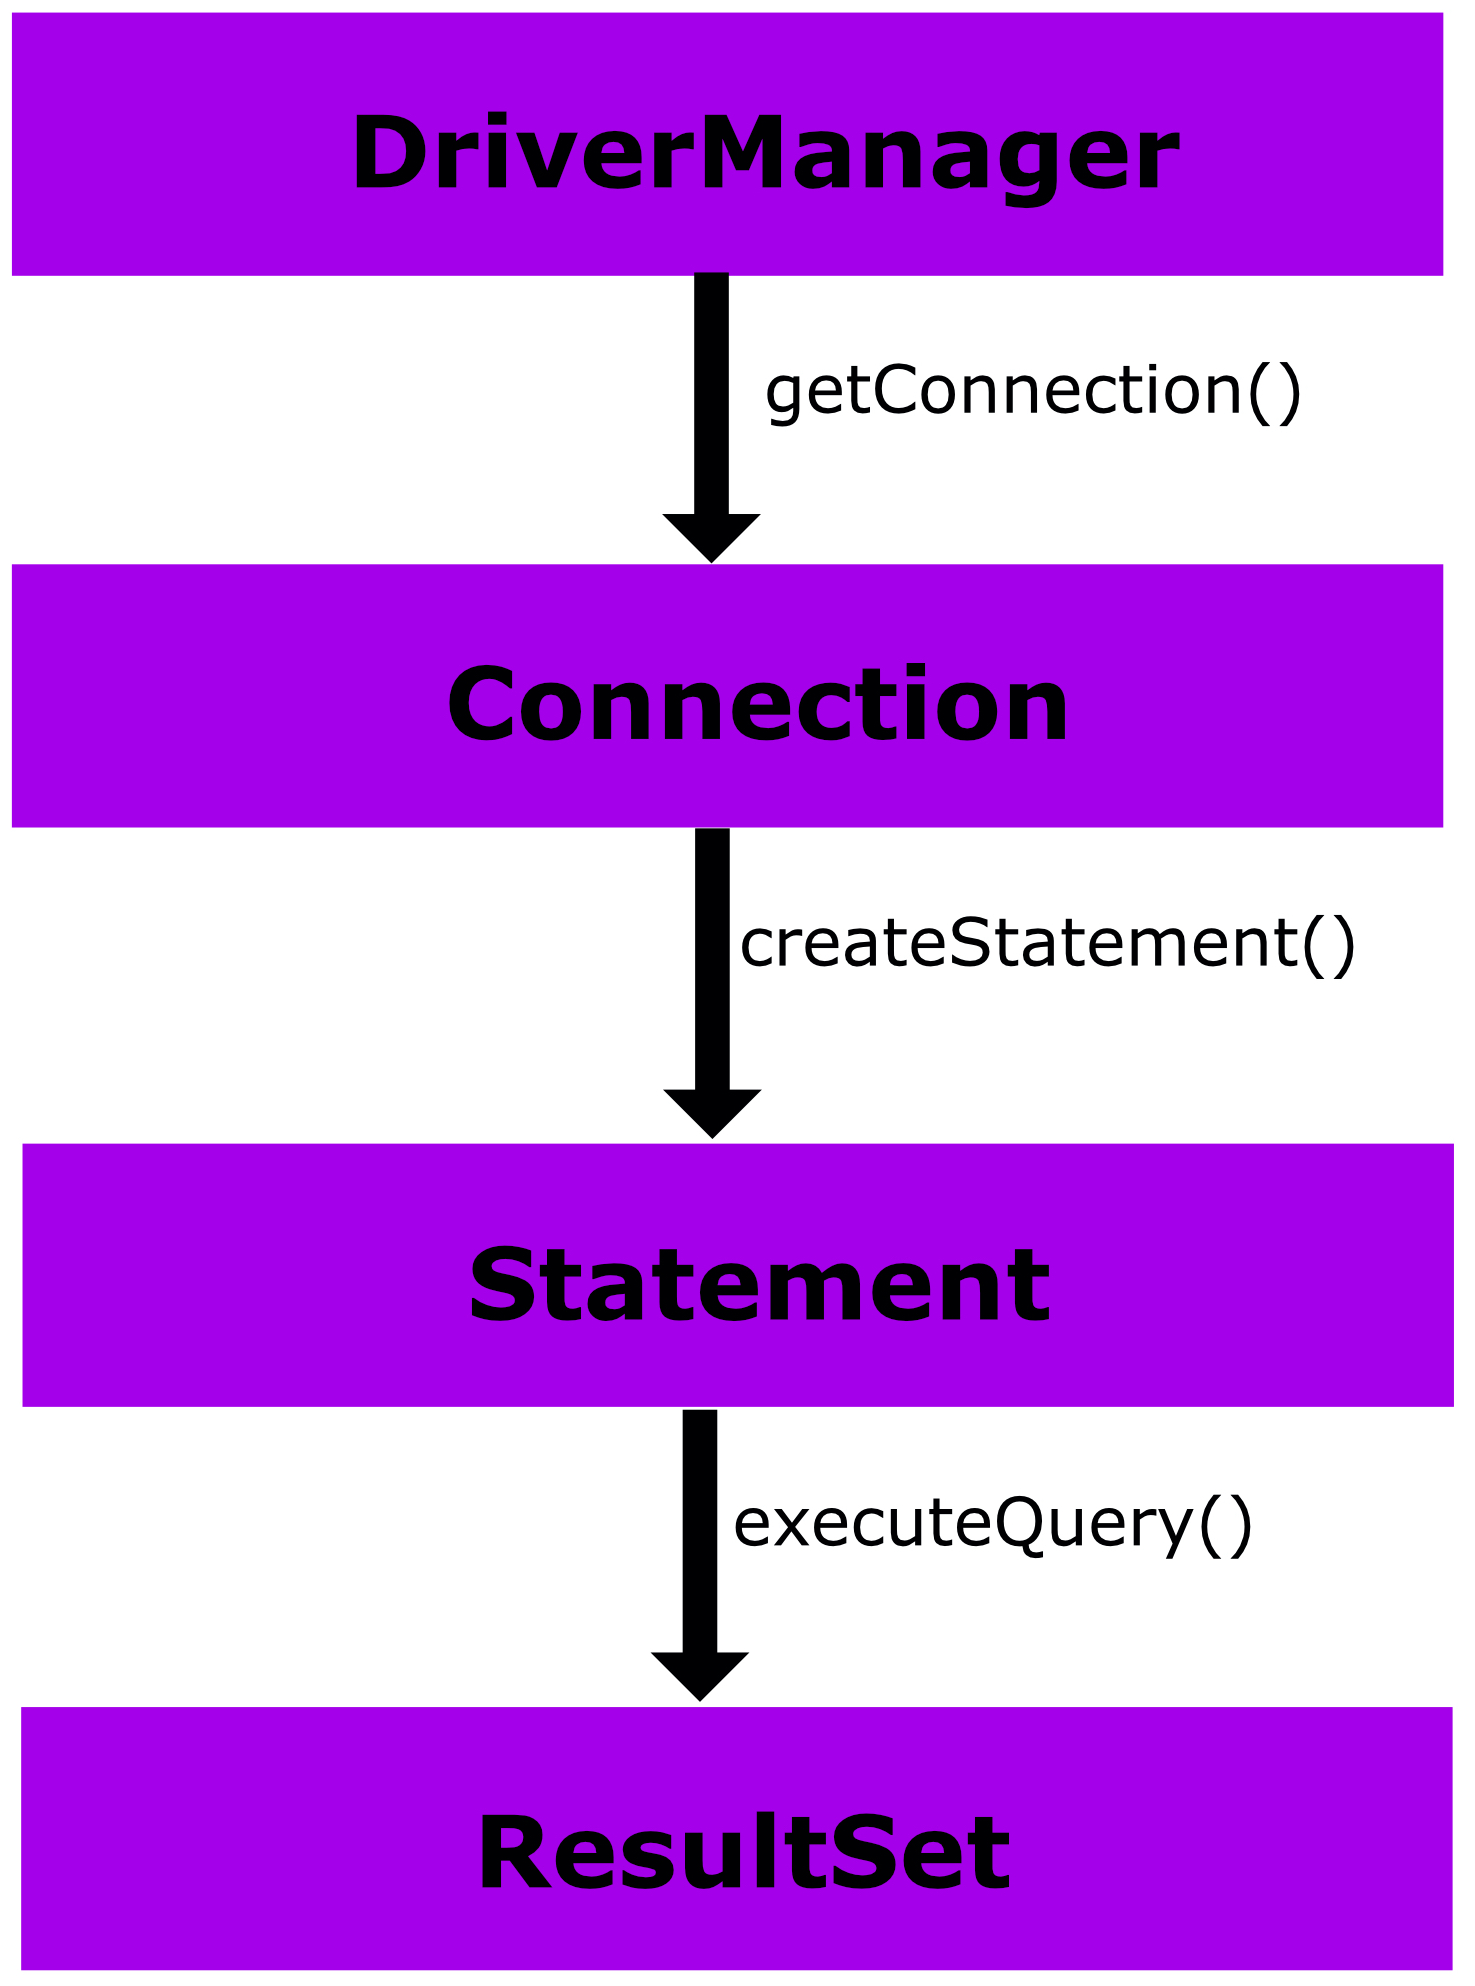
\includegraphics[width=0.35\linewidth]{./img/Connection.jpg}
  		\caption{Datenbankverbindung}
  		\label{Datenbankverbindung}
	\end{figure}
	\end{center}
\end{frame}
\begin{frame}
	\frametitle{Ablauf der Datenbankverbindung}
	\framesubtitle{Erklärung}
	\begin{itemize}
		\item Aufbau einer Verbindung zur DB
		\begin{itemize}
			\item Angabe der Verbindungsinformationen
			\item Auswahl und dynamisches Laden des Treibers
		\end{itemize}
	\item Senden einer SQL-Anweisung
		\begin{itemize}
			\item Definition der Anweisung
			\item Belegung von Parametern
		\end{itemize}
	\item Verarbeiten der Anfrageergebnisse
		\begin{itemize}
			\item Navigation über Ergebnisrelation
			\item Zugriff auf Spalten
		\end{itemize}
	\end{itemize}
\end{frame}

\begin{frame}
	\frametitle{Ablauf der Datenbankverbindung}
	\framesubtitle{Sourcecode}
	\begin{center}
		%Download here $\ldots$
		\textbf{Netbeans}
	\end{center}
\end{frame}

\begin{frame}
	\frametitle{Datentypen}
	\framesubtitle{Typabbildung MySQL $\rightarrow$ Java}
	\begin{center}
	\begin{figure}
  		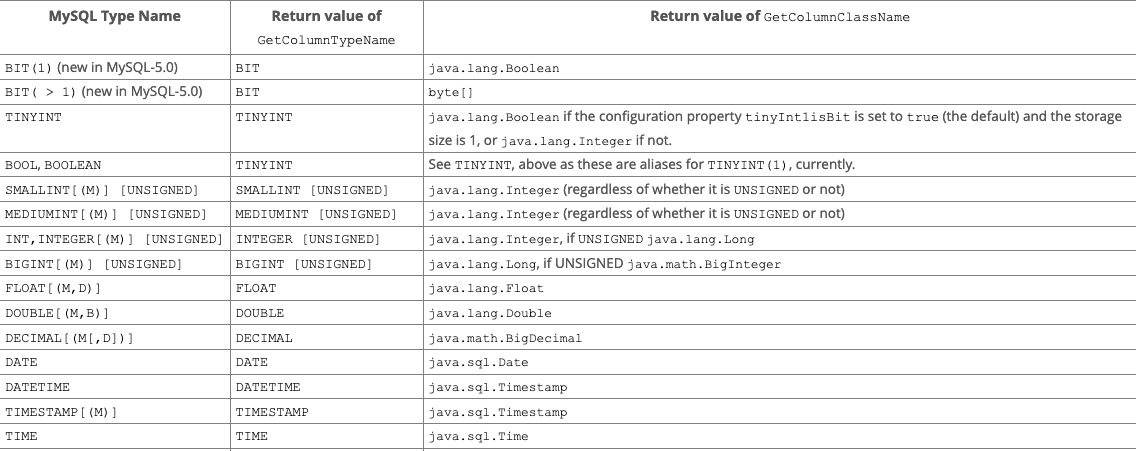
\includegraphics[width=0.9\linewidth]{./img/mapings}
  		\caption{Auszug Typabbildung}
  		\label{Auszug Typabbildung}
	\end{figure}
		\small{Der Link zur gesamten Liste \url{https://bit.ly/2uA5quV}}
	\end{center}
\end{frame}

\section{Exkurs Design Patterns}
\subsection{Was sind Design Patterns}

\begin{frame}
\frametitle{Definition}
\framesubtitle{Entwurfsmuster, Architekturmuster und konkreter Architektur}
	\begin{block}{%Entwurfsmuster, Architekturmuster und konkreter Architektur
	}
		Während eine \textbf{konkrete Architektur} neben der Erfüllung nicht funktionaler Eigenschaften auch \textbf{konkreten funktionalen Anforderungen} genügt, stehen bei einer Referenzarchitektur und bei einem \textbf{Architekturmuster} bzw. \textbf{Entwurfsmuster} die nicht funktionalen Anforderungen  wie \textbf{Standardisierung, Verständlichkeit, Einfachheit} und \textbf{Ausbaufähigkeit} im Vordergrund. \cite{architektur}
	\end{block}
	
	Solche Muster sind nicht auf Java beschränkt, sondern können bei allen objektorientierten Sprachen angewendet werden.	
\end{frame}

\begin{frame}
\frametitle{Entwurfsmuster}
	\begin{block}{Definition Entwurfsmuster}
		In der objektorientierten Softwareentwicklung sind \textbf{Entwurfstmuster Klassen in Rollen,} die zusammenarbeiten, um \textbf{gemeinsam} eine \textbf{bestimmte Aufgabe} zu \textbf{lösen}.\cite{architektur}	\end{block}
\end{frame}

\begin{frame}
\frametitle{Entwurfsmuster vs. Architekturmuster}
	\begin{block}{Unterschied Architekturmuster und Entwurfsmuster}
		\textbf{Entwurfsmuster} stellen \textbf{feinkörnige Muster} dar, während \textbf{Architekturmuster grobkörnige Muster} sind. \cite{architektur}
	\end{block}
\end{frame}

\begin{frame}
\frametitle{Einige Beispiele}
	\textbf{Entwurfsmuster:} 
	\begin{itemize}
		\item Visitor Pattern
		\item Factory Pattern
		\item Singleton Pattern
	\end{itemize}
	\vspace{0.3cm}
	\textbf{Architekturmuster:} 
	\begin{itemize}
		\item MVC $\ldots$ Model View Controller
		\item Schichtenarchitektur
		\item Client-Server
	\end{itemize}
\end{frame}

\subsection{Singleton Pattern}

\begin{frame}
\frametitle{Definition}
%\framesubtitle{Definition}
\begin{block}{Definition Singleton}
	Das \textbf{Singleton-Muster} soll gewährleisten, dass eine Klasse nur ein einziges Mal instanziert werden kann. \cite{architektur}
\end{block}

\end{frame}

\begin{frame}
	\frametitle{Beispiel}
	%\framesubtitle{Beispiel}
\begin{alertblock}{Problem}
	Es soll eine Klasse geben, von der sichergestellt werden muss, dass nur eine einzige Instanz von ihr existiert. Für das Erzeugen der einzigen Instanz soll die genannte Klasse selbst verantwortlich sein. \cite{architektur}
\end{alertblock}
\end{frame}

\begin{frame}
	\frametitle{Beispiel}
	%\framesubtitle{Beispiel}
\begin{exampleblock}{Lösung}
	Ein Singleton Objekt kann nur von der Klasse \textit{Singleton} selbst erzeugt werden. Alle Konstruktoren dieser Klasse werden mit dem Zugriffsmodifier \textit{private} gekennzeichnet, so dass andere Klassen kein Objekt unter Verwendung eines Konstruktors erzeugen können. Objekte, die die Klassen \textit{Singleton} verwenden möchten, erhalten von der Klassenmethode \textit{getInstance()} der Klasse \textit{Singleton} eine Referenz auf das einzig existierende Objekt der Klasse \textit{Singleton} zurück. \cite{architektur}
\end{exampleblock}
\end{frame}

\begin{frame}
	\frametitle{UML Diagramm}
	%\framesubtitle{UML Diagramm}
\begin{center}
	\begin{figure}
  		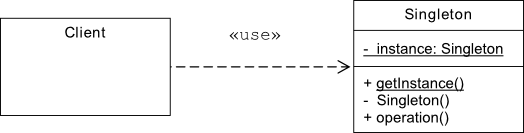
\includegraphics[width=0.9\linewidth]{./img/uml}
  		\caption{UML Diagramm Singleton}
  		\label{UML Diagramm Singleton}
	\end{figure}
	\cite{architektur}
	\end{center}
\end{frame}

\subsection{Singleton und JDBC}

\begin{frame}
	\frametitle{Sourcecode}
	\framesubtitle{}
	\inputminted{java}{/Users/lukas/NetBeansProjects/SQLApplication/src/sqlapplication/Singleton.java}	
	\end{frame}

\section{Zugangsdaten}
\begin{frame}
	\frametitle{Setup der Datenbank}
	\framesubtitle{}
	\begin{itemize}
		\item username: codersbay
		\item password: codersbay
		\item Link zu phpmyAdmin \url{https://www.db4free.net/phpMyAdmin/}
		\item Download Connector/J 8.0.19 für MySQL 
		\url{https://dev.mysql.com/downloads/connector/j/}
		
		\item \colorbox{orange}{\textbf{Link für Java}}\\ "jdbc:mysql://db4free.net:3306/codersbayworld?\\zeroDateTimeBehavior=CONVERT\_TO\_NULL"
	\end{itemize}
\end{frame}
\section{Abschluss}
\begin{frame}
\frametitle{Verwendung von JDBC}
	\begin{block}{SQL Statements in Java}
		SQL Statements sollten aus Performancegründen sehr sparsam eingesetzt werden. Nach Möglichkeit das Datenbankmanagementsystem DBMS verwenden. \\
		\textbf{Cursor, Trigger, PLSQL, Exceptions, $\ldots$ .}
	\end{block}

\end{frame}

\begin{frame}
\frametitle{Referenzen}
        \bibliographystyle{ieeetr}
        \bibliography{bibfile.bib}
\end{frame}

\end{document}